\chapter {Adaptation de BSO aux problèmes d'optimisation continue}

\section* {Introduction}
L'objectif de notre travail est d'adapter la méta-heuristique BSO aux problèmes d'optimisation continue sans trop affecter sa structure initiale. Après un rappel du principe général de BSO, nous passons en revue les domaines dans lesquels elle a été appliquée. Puis, nous exposons notre contribution qui consiste à son adaptation à l'optimisation continue.

\section{L'algorithme Bee Swarm Optimization (BSO)}

\subsection{Principe}

L’algorithme BSO classique s’inspire du comportement naturel des essaims
d'abeilles.

L'abeille éclaireuse quitte la ruche à la recherche du nectar. Quand
elle le trouve, elle revient à la ruche avec un peu de récolte, puis elle fait une danse circulaire. Pour les sources de nourriture qui sont loin de la ruche, l'abeille éclaireuse change petit à petit sa danse en une danse en huit (la danse d'abeille est riche en informations parce qu'elle indique la
quantité de la nourriture trouvée, la distance qui la sépare de la ruche et la direction de sa source).

L'essaim d'abeilles se dirige vers la source de nourriture la plus riche,
même si elle est la plus éloignée (ce comportement a été confirmé par
l'expérience de Seeley et ses camarades \cite{seeley1991collective}).

Du point de vue informatique, on associe à l'abeille
éclaireuse un sommet de référence qui est une solution construite
aléatoirement ou en suivant une heuristique. A partir de ce sommet, on
génère $n$ autres solutions en utilisant le paramètre $Flip$ permettant de déterminer un ensemble de points de l'espace de recherche à explorer. L’ensemble de
ces solutions définit la zone de recherche.

Ensuite, on attribue chaque point ou solution de la zone de recherche à une abeille, qui fera une recherche locale afin d’aboutir à un optimum local. L'ensemble des optimums locaux est mis dans une table appelée $Danse$. Le meilleur optimum local à une itération sera considéré comme le nouveau sommet de référence de la prochaine itération.

Pour éviter de boucler indéfiniment dans la même zone de
l’espace de recherche, le sommet de référence est sauvegardé à chaque
fois dans une liste appelée $Tabou$.

Dans un premier temps, le choix du sommet de référence est fait en
se basant sur les qualités des solutions (phase d’intensification). Puis, si après
une certaine période de temps, on n'arrive pas à améliorer la solution, on
utilise le critère de diversité pour changer de région et en explorer d’autres (phase de diversification).\\

L’algorithme BSO est le suivant:

\begin{algorithm}
	\caption{BSO}
	\KwIn{Les paramètres de l'algorithme et la condition d'arrêt}
	\KwOut{La meilleure solution trouvée}
	\Begin{
    Soit $Sref$ la solution trouvée par l'abeille éclaireuse\;
    \While{la condition d'arrêt est non vérifiée}{
      Insérer $Sref$ dans la liste $Tabou$\;
      Déterminer la zone de recherche à partir de $Sref$\;
      Attribuer une solution $s$ de la zone de recherche à chaque abeille\;
      \For{chaque abeille}{
        Recherche locale avec la solution $s$\;
        Mettre l'optimum local dans la table $Danse$\;
      }
      Choisir le nouveau sommet de référence $Sref$\;
    }
  }
\end{algorithm}

\subsection{Applications}

C'est en 2005 que l’algorithme BSO a été proposé et appliqué sur le problème de satisfiabilité MAXW-SAT puis adapté à plusieurs domaines d’application parmi lesquelles la fouille de données et la recherche d’information \cite{DRIAS_SADEG_YAHI_2005}.

Une méthode hybride a été proposée pour prendre en charge les instances volumineuses du problème SAT.
Cette méthode se base essentiellement sur la méta-heuristique bio-inspirée BSO et sur le paradigme multi-niveaux. Dans ce travail, on perçoit l’importance de la combinaison de deux approches prometteuses afin de bénéficier de leurs avantages \cite{DJEFFAL_DRIAS_2013}.

Une combinaison entre le Clustering (une tâche du Data Mining) et la méta-heuristique BSO a été mise au point pour améliorer l’efficacité de la résolution du problème
SAT. L’approche suivie consiste à explorer judicieusement l’espace de
recherche avant de lancer le processus de recherche de solutions qui va
réduire la complexité des instances volumineuses du problème SAT. Deux
méthodes ont été proposées. La première consiste à intégrer le Clustering
dans la structure originale de BSO, qui va mener à suggérer une version
avancée de BSO. La deuxième méthode consiste à faire un Clustering sur
les données avant de lancer BSO. Cette manière de procéder aide à
réduire le nombre de clauses et le nombre de variables des instances SAT
et donc le temps d'exécution \cite{DRIAS_DOUIB_HIRECHE_2013}.

D'autres auteurs ont proposé un nouvel algorithme de
recherche de règles d'association basé sur une version améliorée de BSO
avec trois heuristiques différentes pour explorer l'espace de recherche.
Cette approche a été implémentée et testée sur différentes bases de
données de petite, moyenne et grande taille. Les résultats obtenus
montrent que l'approche proposée est meilleure que certains algorithmes
de la littérature en termes de qualité et de temps d'exécution \cite{DJENOURI_DRIAS_HABBAS_2014}.

Nous nous intéressons dans ce travail à l'adaptation de BSO aux problèmes d'optimisation continue afin d'élargir son champ d'application. Nous allons présenter notre contribution à cette problématique en développant une version de BSO pour les problèmes à variables continues, que nous avons appelée Continuous Bee Swarm Optimization (CBSO).

\section{Continuous Bee Swarm Optimization (CBSO)}
Le problème que nous traitons consiste en des fonctions
mathématiques à plusieurs dimensions (variables). A noter que la fonction problème est elle-même la fonction objectif qu'on cherche à minimiser. Le but est donc de trouver les valeurs réelles que prennent les variables ($x_1, x_2,..., x_n$ où $n$ est la dimension du problème) pour lesquelles la fonction donne l'image la plus petite possible (les bornes inférieures de la fonction). Cette tâche n'est pas évidente vu que la représentation graphique d'une fonction est impossible si elle comporte plus de deux variables.

De plus, l'inexistence de méthodes analytiques (comme le calcul de dérivée) rapides pour trouver des solutions à ce genre de problèmes donne importance aux méta-heuristiques de l'optimisation continue en général.\\

La difficulté par rapport aux problèmes d'optimisation combinatoire,
c'est qu'une variable (dimension du problème) peut prendre une
infinité de valeurs possibles dans son domaine de définition, ce qui va
rendre son voisinage étroit. Donc, il n'est pas pratique d'utiliser les
mêmes démarches que pour un algorithme d'optimisation combinatoire pour
trouver la solution souhaitée.

Pour pallier ce problème, il nous faut définir de nouvelles techniques adéquates. Notons que toutes les valeurs présentées des paramètres de l'algorithme ont été obtenues après plusieurs expérimentations.

\subsection{Voisinage d'une solution}
Soit $[a,b]^n$ le domaine de définition d'une fonction d'optimisation continue à $n$ variables. Pour définir le voisinage d'une solution $s$, nous nous sommes inspirés de la méthode de N. Hu \cite{Hu_1992} qui se base sur le principe de disque.

Soit $B(s,r)$ le disque centré par $s$ avec un rayon $r$, il contient l'ensemble des points $s'$ tels que $\Vert s'- s\Vert \leq r$. Le symbole $\Vert \cdot\cdot\cdot \Vert$ est utilisé pour dénoter la norme euclidienne.

Pour une exploration homogène de l'espace de recherche, N. Hu considère un ensemble de disques centrés par la solution $s$, avec des rayons respectifs $h_0,h_1,...,h_k$. Par conséquent, l'espace est partitionné en $k$ couronnes concentriques:

$$C_j(s,h_{j-1},h_j)=\{s'\vert h_{j-1}\leq \Vert s'-s\Vert \leq h_j\}\quad , \quad 1 \leq j \leq k $$.

A partir de ces couronnes, $k$ voisins de $s$ sont extraits, chacun à partir d'une couronne $C_j$, et cela en faisant une sélection aléatoire d'un point à l'intérieur de chaque couronne $C_j$, pour $j$ variant de $1$ à $k$.

Le rayon $h_k$ du plus grand disque est un paramètre de l'algorithme. Les autres rayons $h_j$ ($1\leq j\leq k-1$) sont calculés à partir de $h_k$,  selon la méthode de partitionnement géométrique suivante:

$$
h_{k-j+1}=\frac{h_k}{2^{j-1}}, j=2,...,k.
$$

Le rayon $h_0$ est un autre paramètre de l'algorithme qui satisfait la condition:

$$
h_0<\frac{h_k}{2^{k-1}}.
$$

Le partitionnement de l'espace autour de $s$ dépend donc du nombre $k$ de voisins, du rayon $h_k$ du disque externe et du rayon $h_0$ du disque interne.

Dans CBSO, nous avons adopté le principe de calcul des rayons $h_0,h_1,...,h_k$, mais nous traitons chaque variable de la solution $s$ indépendamment des autres. C'est pourquoi ques nous devons d'abord introduire le voisinage d'une variable.

\subsubsection{$\bullet\quad$Voisinage d'une variable}
Soient $X_i$ la $i^{ème}$ variable de la solution $s$ et $x_i$ la valeur de cette variable. Notons cette variable ($X_i$, $x_i$).  Le partitionnement du voisinage de $s$ pour la variable $X_i$ se fait comme suit:

\vspace{-1em}

\begin{figure}[H]
	\centering
	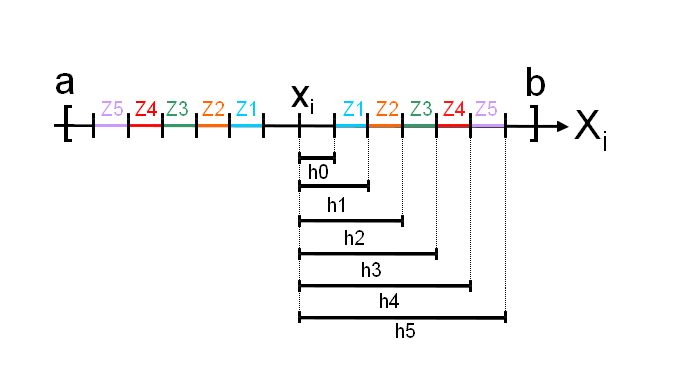
\includegraphics[width=0.7\textwidth,keepaspectratio]{partitionnement_voisinage_CBSO}
	\caption{Partitionnement du voisinage dans CBSO}
\end{figure}


Une zone uni-dimensionnelle $Z_j$ définie par les rayons $h_{j-1}$ et $h_j$ est composée de deux parties égales, une à gauche de $x_i$ et une à droite de $x_i$.

Une variable ($X_j$, $x_j$) est voisine de la variable ($X_i$, $x_i$) si et seulement si elle appartient à une des $k$ zones uni-dimensionnelles. Autrement dit:

$$
|x_i - x_j|\leq h_k
$$

Une variable ($X_j$, $x_j$) n'est pas voisine de la variable ($X_i$, $x_i$) si et seulement si elle n'appartient à aucune des $k$ zones uni-dimensionnelles. Autrement dit:

$$
|x_i - x_j|> h_k
$$ 

\subsubsection{$\bullet\quad$Voisinage d'une solution}
Soit $V$ le symbole dénotant la notion de voisinage. Une solution $s'$ est voisine de la solution $s$ si et seulement si toutes les variables de $s'$ sont voisines de celles de $s$:

$$
s' \in V(s) \Leftrightarrow x'_i \in V(x_i) , \forall i=1,...,n
$$

Une solution $s'$ n'est pas voisine de la solution $s$ si et seulement si toutes les variables de $s'$ ne sont pas voisines de celles de $s$:

$$
s' \notin V(s) \Leftrightarrow x'_i \notin V(x_i) , \forall i=1,...,n
$$

Il est important de s'assurer que les coordonnées de la solution voisine ou non-voisine de $s$ appartiennent au domaine de définition [a,b]. Pour cela, il faut s'assurer que la plus grande zone ne dépasse pas le domaine de définition de la fonction. Autrement dit, le paramètre $h_k$ doit vérifier la contrainte suivante:

$$ 
h_k < \frac{b-a}{2}.
$$

\subsubsection{$\bullet\quad$Détermination d'une solution voisine}

Cela consiste à déterminer les $n$ coordonnées d'une solution $s'$ (une par une) dans la zone définie par les rayons $h_{j-1}$ et $h_j$.

Dans le cas où la valeur $x_i$ de la variable $X_i$ se trouve au milieu du domaine $[a,b]$, il suffit que le générateur de nombres aléatoires choisisse une valeur $x'_i$, telle que:

$$
x'_i\in[x_i-h_{j+1},x_i-h_j] \cup [x_i+h_j,x_i+h_{j+1}]
$$

où:
\begin{itemize}
	\item $x_i$ est la $i^{ème}$ coordonnée de la solution $s$,
	\item $x'_i$ est la $i^{ème}$ coordonnée de la solution voisine.\\
\end{itemize}

Il se peut que la valeur $x_i$ de la variable $X_i$ soit proche de l'une des deux frontières du domaine de définition de la fonction (Figure \ref{debordement}). Dans ce cas, une partie (hachurée) des $k$ zones débordera du domaine [a,b], et seulement l'autre partie (non-hachurée) sera valide et pourra être utilisée pour générer la coordonnée $x'_i$ de la solution non voisine. 

\vspace{-1em}

\begin{figure}[H]
	\centering 
	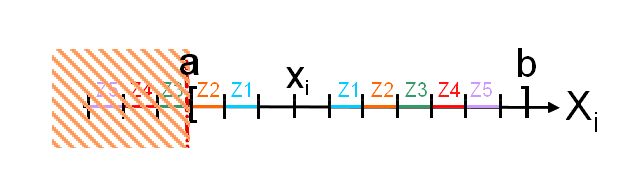
\includegraphics[width=0.7\textwidth,keepaspectratio]{debordement_voisinage2}
	\caption{Débordement du voisinage d'une variable} 
	\label{debordement}
\end{figure}

Si les zones débordent de la borne inférieure, le générateur de nombres aléatoires choisit la valeur $x'_i$ telle que:

$$
x'_i\in[x_i+h_j,x_i+h_{j+1}]
$$

Si les zones débordent de la borne supérieure, le générateur de nombres aléatoires choisit la valeur $x'_i$ telle que:

$$
x'_i\in[x_i-h_{j+1},x_i-h_j]
$$

\subsubsection{$\bullet\quad$Détermination d'une solution non voisine}

Cela consiste à déterminer les coordonnées d'une solution en dehors des $k$ zones.

Dans le cas où la valeur $x_i$ de la variable $X_i$ se trouve au milieu du domaine $[a,b]^2$, il suffit que le générateur de nombres aléatoires choisisse une valeur $x'_i$, telle que:

\begin{equation}
x'_i\in[a,x_i-h_k] \cup [x_i+h_k,b],\label{for1}
\end{equation}

Si les zones débordent de la borne inférieure, alors le générateur de nombres aléatoires choisit la valeur $x'_i$ telle que:

\begin{equation}
x'_i\in[x_i+h_k,b],\label{for2}
\end{equation}

Si les zones débordent de la borne supérieure, le générateur de nombres aléatoires choisit la valeur $x'_i$ telle que:

\begin{equation}
x'_i\in[a,x_i-h_k],\label{for3}
\end{equation}


\parbox[t][]{\textwidth}{}

\vspace{-2.5em}

\subsection{Distance entre deux solutions}
\begin{spacing}{1.6}
Nous avons besoin de cette notion pour le calcul de diversité lors de la phase de diversification. Pour répondre à notre besoin, nous avons choisi la norme $infini$ qui considère le maximum des différences entre les coordonnées des deux solutions. Elle est donnée par la formule:
\end{spacing}

\vspace{0.25em}

$$
Distance(s,s')=\Vert s-s'\Vert_\infty=Max\{\vert x_{1i}-x_{2i} \vert\}, \quad 1\leq i \leq n
$$

\vspace{2em}

où:
\begin{itemize}
	\item $\Vert \cdot \cdot \cdot \Vert_\infty$ est la norme $"infini"$,
	\item $s$ et $s'$ sont deux solutions,
	\item $n$ est la dimension de la fonction problème (le nombre de variables),
	\item $x_{1i}$ est la $i^{ème}$ variable de la première solution,
	\item $x_{2i}$ est la $i^{ème}$ variable de la deuxième solution.\\
\end{itemize}

Par cela, nous définissons notre propre manière de voir la distance entre deux solutions.

\subsection{Diversité d'une solution}

C'est une valeur réelle que nous calculons pour chaque solution de la table $Danse$. Elle est donnée par la formule suivante:

\vspace{-1em}

$$
Diversité(s)= Min\{\Vert s-s' \Vert_\infty , \forall s' \in Tabou\}.
$$


Cette mesure permet d'indiquer à quel point la solution $s$ est éloignée des sommets de référence des itérations précédentes. Rappelons que la liste $Tabou$ contient les anciens sommets de référence.

\vspace{-1em}

\subsection{Algorithme}

\begin{algorithm}[H]
	\caption{CBSO}
	\KwIn{Les paramètres de l'algorithme et la condition d'arrêt}
	\KwOut{La meilleure solution trouvée}
	\Begin{
    Soit $Sref$ la solution trouvée par l'abeille éclaireuse\;
    \While{la condition d'arrêt est non vérifiée}{
      Insérer $Sref$ dans la liste $Tabou$\;
      Déterminer la zone de recherche à partir de $Sref$\;
      Attribuer une solution $s$ de la zone de recherche à chaque abeille\;
      \For{chaque abeille}{
        Recherche locale avec la solution $s$\;
        Mettre l'optimum local dans la table $Danse$\;
      }
      Construire la solution noyau et l'insérer dans la table $Danse$\;
      Choisir le nouveau sommet de référence $Sref$\;
    }
  }
\end{algorithm}

\bigskip

Nous pouvons constater que notre algorithme ne change pas la structure générale de l'algorithme BSO sauf que chaque étape est définie de manière à être mieux adaptée aux problèmes continus.

\subsubsection{$\bullet\quad$Génération du sommet de référence initial}
\begin{spacing}{1.6}
Le sommet de référence initial est construit d'une manière incrémentale (variable par variable). A chaque variable de $Sref$, le générateur de
nombres aléatoires attribue une valeur réelle aléatoire qui obéit à la loi uniforme donnée par la formule suivante:

\begin{equation}
u(x) = \left\{ \begin{array}{rcl}
	\frac{1}{b-a} & \mbox{si}
	& x\in [a,b] \\ 0 & \mbox{sinon}
\end{array}\right.\label{eq2}
\end{equation}


Toutes les valeurs réelles appartenant à l'intervalle $[a,b]$ ont la même probabilité ($p=\frac{1}{b-a}$) d'être choisies et aucune autre valeur ne sera choisie ($p=0$).\\

\subsubsection{$\bullet\quad$Détermination de la zone de recherche}
Elle consiste à générer $m$ solutions à partir du sommet de référence ($m$ étant le nombre d'abeilles) et à attribuer une solution à chaque abeille pour démarrer la recherche locale.

Nous avons considéré quatre abeilles dont les solutions sont distribuées comme suit,

\begin{itemize}
	\item la première abeille travaille sur le sommet de référence. Cela signifie qu'à partir de la deuxième itération, elle va continuer le travail des abeilles de l'itération précédente ($intensifier$ encore plus la recherche),
	\item la deuxième abeille travaille sur une solution non voisine du sommet de référence, pour $diversifier$ la zone de recherche. Cette solution est déterminée en utilisant une des formules \ref{for1}, \ref{for2} ou \ref{for3},
	\item En utilisant le paramètre $Flip$, la troisième abeille combine entre le sommet de référence et une solution non voisine de telle manière à obtenir une \emph{solution hybride}. Nous avons choisi $Flip=2$ ce qui signifie que cette abeille prend les cases impaires du sommet de référence et les cases paires de la solution non voisine.
	
	\vspace{1em}

	\begin{figure}[H]
		\centering
		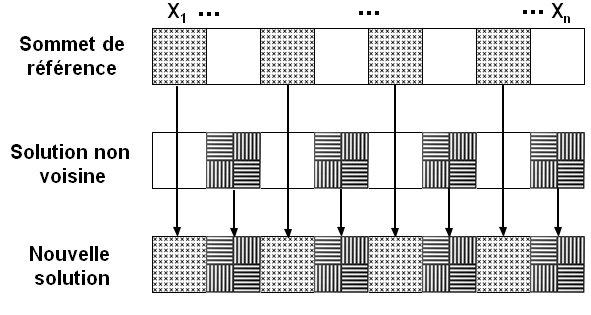
\includegraphics[width=0.8\textwidth,keepaspectratio]{construction_solution}
		\caption{Construction d'une solution à partir de Sref et d'une solution non voisine}
	\end{figure}

	\parbox[][0.5em]{\textwidth}{}

	L'algorithme de construction de la nouvelle solution hybride en utilisant le paramètre $Flip$ est donné comme suit:\\
	
\end{itemize}
	
	\begin{algorithm}[H]
		\KwIn{$Sref$, solution non voisine et $Flip$}
		\KwOut{La nouvelle solution hybride}
		\Begin{
		
				solutionHybride$\leftarrow Sref$\;
				$i\leftarrow Flip$\;
				\While{$i\leq n$}{
					solutionHybride[i]$\leftarrow$ solutionNonVoisine[i]\;
					$i\leftarrow i+Flip$\;
			}
		}
		\caption{Construction de la nouvelle solution}
	\end{algorithm}
\vspace{3em}

\begin{itemize}
	\item la quatrième abeille fait de même que pour la troisième abeille, sauf que la solution obtenue prend les cases paires du sommet de référence et les cases impaires de la solution non voisine.
\end{itemize}
\end{spacing}

\vspace{-0.5em}

\subsubsection{$\bullet\quad$Recherche locale}

\vspace{-0.5em}

Après avoir attribué les solutions de la zone de recherche aux abeilles, chacune d'elles démarre une recherche locale avec sa solution en explorant son voisinage pour éventuellement choisir le voisin qui minimise le plus la fonction objectif.

Après plusieurs expérimentations, nous avons choisi d'opter pour le voisinage en étoile basé sur les deux étapes suivantes:
\begin{itemize}
	\item Générer 5 voisins ($k=5$) tels que les coordonnées de chaque voisin sont prises d'une zone différente ($Z_1,Z_2,...,Z_5$) pour une exploration judicieuse de l'espace de recherche.
	\item Comparer les $k$ voisins générés deux à deux, puis prendre le meilleur et le comparer avec la solution $s$. S'il est meilleur, il sera considéré comme l'optimum local pour cette abeille à cette itération, sinon, la solution $s$ le sera.
\end{itemize}

Le processus de recherche locale est répété un nombre de fois défini par le paramètre $SearchIter$.

\vspace{0.5em}

\begin{algorithm}[H]
	\caption{Recherche locale}
	\KwIn{Solution $s$, $SearchIter$ et $k$}
	\KwOut{Optimum local}
	\Begin{
    \For{$i$ allant de $1$ \KwTo $SearchIter$}{
      \For{$j$ allant de $1$ \KwTo $k$}{
        Générer un voisin $v_i$ dans la $j^{ième}$ zone\;
        \uIf{fitness($v_i$)$ \leftarrow optimum$}
        {
          $\quad\quad$ Retourner $v_i$\;
        }
        \ElseIf{$v_i$ est le meilleur voisin}
        {
          $\quad\quad meilleur\_voisin \leftarrow v_i$\;
        }

      }
      \uIf{fitness($meilleur\_voisin$) $\leq$ fitness($s$)}
      {
        $\quad\quad$Retourner $meilleur\_voisin$\;
      } \Else {Retourner $s$\;}
    }
  }
\end{algorithm}

A la fin de la recherche locale, chaque abeille communique son optimum local à travers la table $Danse$. Celle-ci va donc contenir à la fin de chaque itération, les sommets de référence potentiels de la prochaine itération.

\begin{spacing}{1.4}

\subsubsection{$\bullet\quad$Construction de la solution noyau}

En plus des $m$ optimums locaux existant dans la table $Danse$, nous construisons, à partir de la même table, une autre solution que nous appelons \emph{solution noyau}. Nous nous sommes inspirés de ACO$_\mathbb{R}$ \cite{SOCHA_DORIGO_2006} pour construire cette solution en faisant un choix probabiliste sur ses $n$ composants.

\vspace{1em}

Pour cela, nous utilisons la fonction gaussienne noyau (Gaussian kernel) qui est une distribution de probabilités continue construite à partir de $n$ fonctions gaussiennes individuelles associées aux solutions de la table $Danse$.
\end{spacing}

\parbox[t][1em]{\textwidth}{}

Pour chaque dimension $i$ du problème, il existe une fonction gaussienne noyau $G^i$ différente dont la formule est la suivante:

$$
G^i (x) = \sum^{m}_{j=1} \omega_j \frac{1}{\sigma^i_j \sqrt{2\pi}} \mathrm{e}^{-\frac{(x-\mu^i_j)^2}{2\sigma_j^{i^2}}}
,$$

où:
\begin{itemize}
	\item $m$ est le nombre de solutions dans la table $Danse$,
	\item $\omega_j$ est le poids associé à la $j^{ème}$ solution donné par son rang (la solution qui a la meilleure évaluation aura le plus grand poids et celle qui a la pire évaluation aura le plus petit poids),
	\item $\mu^i$ est le vecteur des moyennes,
	\item $\sigma^i$ est le vecteur des écart-types.\\
\end{itemize} 

\begin{figure}[H]
	\centering
	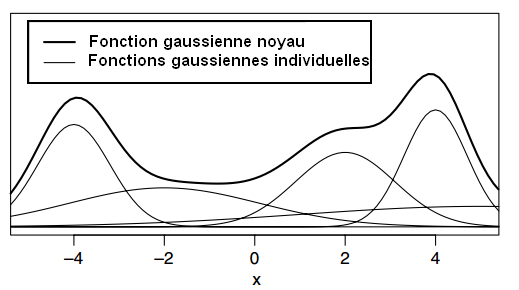
\includegraphics[width=0.8\textwidth,keepaspectratio]{representation_gauss}
	\caption[Représentation graphique de la fonction gaussienne noyau]{Représentation graphique de la fonction gaussienne noyau \cite{SOCHA_DORIGO_2006}}
\end{figure}

La fonction gaussienne noyau nous permet de détecter les régions prometteuses à partir des optimums locaux trouvés par les abeilles. Cela nous aide à nous rapprocher encore de l'optimum global.

Le processus de construction de la nouvelle solution est appelé échantillonnage de la fonction gaussienne noyau et est défini pratiquement, pour chaque dimension $i$ du problème, par:

\begin{itemize}
	\item le choix de la meilleure solution $s_l$ dans la table $Danse$,
	\item le calcul des valeurs $\mu^i_l$ et $\sigma^i_l$ associées à $s_l$,
	\item l'appel au générateur de nombre aléatoires gaussien qui prend en entrée $\mu^i_l$ et $\sigma^i_l$ et retourne une valeur réelle aléatoire $x$ qui obéit à la loi gaussienne $N(\mu^i_l,\sigma^i_l)$ donnée par la formule:
	$$
	g(x)= \frac{1}{\sigma^i_l \sqrt{2\pi}} \mathrm{e}^{-\frac{(x-\mu^i_l)^2}{2\sigma_l^{i^2}}} \quad ,\quad x \in [a,b].
	$$
	 .
\end{itemize} 

$\mu^i_l$ est tout simplement la $i^{ème}$ valeur de la meilleure solution ($\mu^i_l=s^i_l$).

L'écart-type $\sigma^i_l$ représente une erreur moyenne entre la $i^{ème}$ valeur de $s_l$ et celles des autres solutions et se calcule par la formule suivante:

$$
\sigma_l^i = \xi \sum_{j=1}^{m} \frac{|S_j^i - S_l^i|}{m-1}.
$$

où $\xi$ est le paramètre qui contrôle la vitesse de convergence de la solution noyau.

Après la construction de la solution noyau, nous l'évaluons et l'insérons dans la table $Danse$, puis nous choisissons le prochain sommet de référence.

\subsubsection{$\bullet\quad$Choix du nouveau sommet de référence}
Lorsqu'il s'agit des fonctions multi-modales (à plusieurs optimums locaux), il est très important que l'algorithme évite d'être stagné dans un optimum local. Pour cela, il faut utiliser une stratégie de diversification de recherche afin de pouvoir converger vers l'optimum global. 

En réalité, ce sont deux buts contradictoires. D'une part, un algorithme est supposé converger le plus vite possible et d'autre part, il est supposé ne pas converger entièrement vers un optimum local.

Cette contradiction est due au fait q'un algorithme ne peut pas savoir si une région prometteuse mène à un optimum local ou à un optimum global. Le défi est d'établir une balance entre l'efficacité (diversification) et la rapidité (intensification). Cela se traduit par la capacité de choisir le bon prochain sommet de référence à partir de la table $Danse$ qui contient $m+1$ solutions.

Soient:

\begin{itemize}
	\item $Sref_t$ le sommet de référence à l'instant $t$,
	\item $Sref_{t+1}$ le sommet de référence à l'instant $t+1$,
	\item $MSolutionQualité$ la meilleure solution en qualité à l'instant $t$,
	\item $MSolution Diversité$ la meilleure solution en diversité à l'instant $t$.
\end{itemize}

\begin{algorithm}[H]
	\caption{Choix du nouveau sommet de référence}
	\KwIn{La table $Danse$}
	\KwOut{Le nouveau sommet de référence $Sref_{t+1}$}
	\Begin{
		\uIf{fitness($MSolutionQualité$) $\leq$ fitness($Sref_t$)\tcc{La meilleure solution à cette itération est meilleure que $Sref_t$} }
				{
					$\quad\quad Sref_{t+1} \leftarrow MSolutionQualité$\;
					
					$\quad\quad NbChances \leftarrow MaxChances$\;
				}
				\Else
				{
					$\quad\quad$ \tcc{La meilleure solution à cette itération est pire que $Sref_t$}
					
					$\quad\quad NbChances \leftarrow NbChances-1$\;
					
					\uIf{$NbChances > 0$ }
					{
						$\quad\quad Sref_{t+1} \leftarrow MSolutionQualité$\;
					}
				
					\Else
					{	
					$\quad\quad Sref_{t+1} \leftarrow MSolutionDiversité$\;
					
					$\quad\quad NbChances \leftarrow MaxChances$\;	
					}		
				}	
	}
\end{algorithm}
\bigskip

Si la meilleure solution en qualité (celle qui a la plus petite évaluation) est meilleure que le sommet de référence, elle sera considérée comme le prochain sommet de référence. Sinon, elle le sera quand même sauf que nous décrémentons le nombre de chances. Si le nombre de chances devient nul, la meilleure solution en diversité (celle qui a la plus grande diversité) sera considérée comme le prochain sommet de référence et le nombre de chances sera réinitialisé à son maximum.

\begin{itemize}
	\item Lors du choix de la meilleure solution en qualité (instructions $4$ et $10$), si deux solutions ont la même qualité, celle qui a la plus grande diversité sera considérée.
	\item Lors du choix de la meilleure solution en diversité (instruction $12$), si deux solutions ont la même diversité, celle qui a la plus petite évaluation (meilleure qualité) sera considérée. 
\end{itemize} 
 
Il est important que la meilleure solution (en qualité ou en diversité) choisie ne soit pas taboue. Si elle l'est, nous choisissons la prochaine meilleure solution et ainsi de suite. Il peut arriver, même rarement, que toutes les solutions de la table $Danse$ soient taboues. Dans ce cas, le prochain sommet de référence sera généré aléatoirement selon la loi uniforme (équation \ref{eq2}).

\subsubsection{$\bullet\quad$Condition d'arrêt}
Les instructions $5$ à $12$ de l'algorithme CBSO sont répétées jusqu'à ce qu'une de ces trois conditions soient vérifiées: 

\begin{itemize}
	\item l'algorithme converge vers la solution souhaitée ($\vert f-f^* \vert < \epsilon$ où $\epsilon$ est un paramètre de l'algorithme),
	\item le nombre maximum des itérations est atteint, 
	\item une stagnation est détectée (on n'aperçoit pas de changement dans le sommet de référence au bout d'un nombre d'itérations défini par le paramètre $Stag$). 
\end{itemize} 
 
\section*{Conclusion}
Nous avons présenté dans ce chapitre l'adaptation de la méta-heuristique BSO aux problèmes d'optimisation continue. Nous passons à présent à l'implémentation de notre algorithme.
